\chapter{Developer documentation}
\label{ch:impl}

This essay automates Selenium tests in a cloud-native environment using a Go-based Kubernetes operator. This section contains full usage instructions for this Kubernetes operator and in-depth explanations of its features, design philosophy, and supporting technologies.

The Kubernetes operator is a tool that automates the deployment, maintenance, and scaling of Selenium tests in a Kubernetes cluster, which will be covered in this documentation. It makes it simple for DevOps teams and developers to integrate Selenium testing into production workflows, guaranteeing that their cloud-native applications are extensively tested and optimized for performance, scalability, and dependability.

This documentation will provide all the information to know to take advantage of the capabilities of this Go-based Kubernetes operator for Selenium testing, whether you are an experienced Kubernetes developer or are just getting started with cloud-native application development. Therefore, let us get in and get to exploring!

\section{Understanding the underlying technologies}

Understanding the underlying technologies that enable the Go-based Kubernetes operator for Selenium testing is crucial before we go into its specifics. The necessity of introducing these technologies and their importance in the context of developing cloud-native applications will be covered in this section.

Due to its capacity to increase the scalability, agility, and dependability of applications running in a cloud environment, cloud-native application development has grown in popularity in recent years. The use of containerization, which offers a standardized and portable mechanism to bundle and distribute programs, is at the core of this strategy.

Popular container orchestration platform Kubernetes has become the de facto standard for scalably managing containerized applications. In addition to tools for automating these procedures, it offers a complete set of primitives for deploying, scaling, and managing containerized applications.

On the other hand, the open-source testing framework Selenium enables programmers to automate web browser testing for web applications. In the context of continuous integration and continuous delivery (CI/CD) pipelines, in particular, it has evolved into a crucial tool for maintaining the quality and performance of online applications.

It is vital to integrate Selenium testing with Kubernetes to use its advantages in a cloud-native environment. The Go-based Kubernetes operator is helpful in this situation. To automate the deployment and maintenance of Selenium tests in a Kubernetes cluster, a custom controller that extends the Kubernetes API is used.

Understanding the underlying technologies is crucial for successfully operating the Go-based Kubernetes operator for Selenium testing. By doing this, DevOps teams and developers may better understand the utility of this operator and utilize it to improve their processes for creating cloud-native applications.

\subsection{Differences between Virtual Machines and Containers}

Virtual machines and containers are two standard technologies in cloud computing and application deployment. Virtual machines and containers offer isolation and virtualization, but they differ in several important ways. The distinctions between virtual machines and containers are covered in this section.

Software-based simulations of physical devices are known as virtual machines. They execute a whole operating system on top of a hypervisor, emulating the entire hardware stack, including the processor, memory, and storage. Each virtual machine has its own virtualized hardware, operating system, and isolated environment in which it operates. As a result, it is possible to run many operating systems on a single physical machine and achieve total isolation.

On the other hand, containers are a minimal type of virtualization that works at the operating system level. Multiple applications can run on the same operating system instance thanks to containers, which use the host operating system kernel and share resources with other containers. Virtual machines can be replaced by more lightweight and practical containers, which speed up the deployment and scaling of applications.

One of the key distinctions is how virtual machines and containers use their resources. Resource wastage can occur because virtual machines need many resources to replicate a whole hardware stack. Contrarily, containers use resources better because they share the host operating system kernel.

\begin{figure}[H]
	\centering
	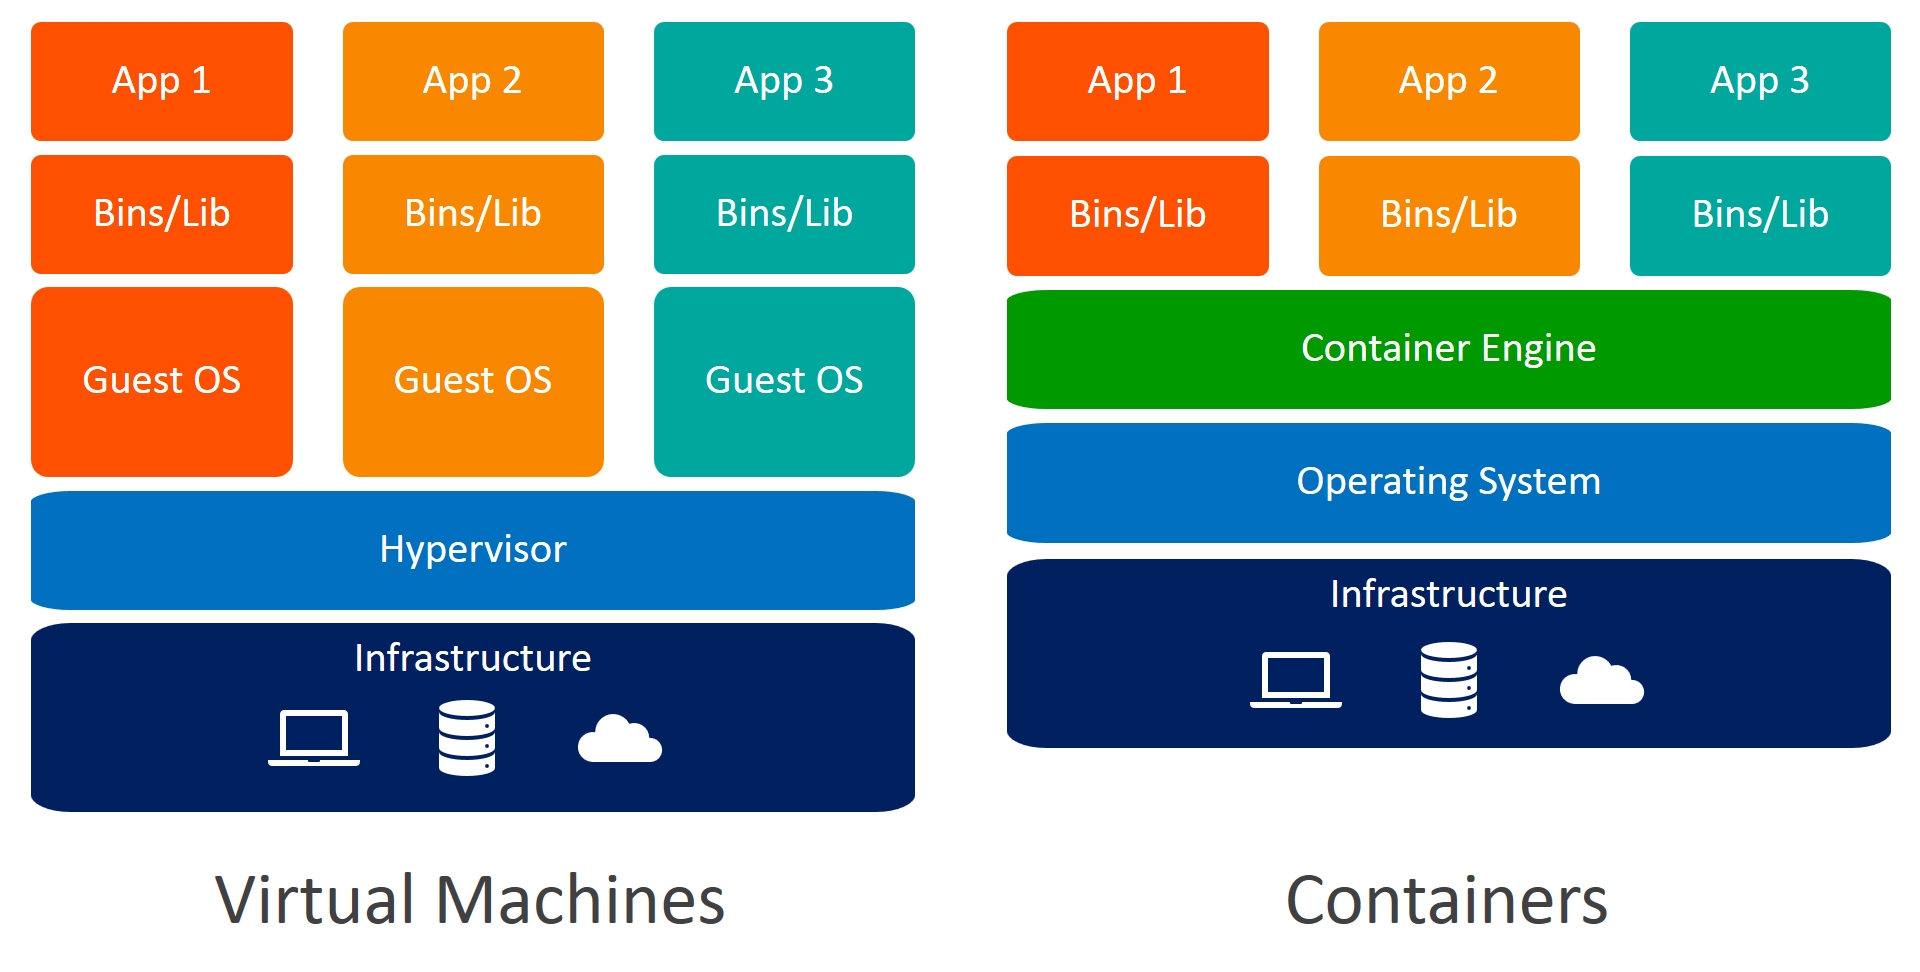
\includegraphics[width=1\textwidth]{containers-vs-virtual-machines}
	\label{fig:container-vs-vm}
\end{figure}

The starting times of virtual machines and containers are another distinction. Virtual machines typically take longer to start up because a complete operating system must be booted. In contrast, containers start up relatively instantaneously because just the containerized program needs to be started.

In conclusion, although virtual machines and containers offer virtualization and isolation, they differ in resource usage, startup time, and security, with containers providing a more portable and practical option for running applications.

\section{Source code samples}

Nulla sodales purus id mi consequat, eu venenatis odio pharetra. Cras a arcu quam. Suspendisse augue risus, pulvinar a turpis et, commodo aliquet turpis. Nulla aliquam scelerisque mi eget pharetra. Mauris sed posuere elit, ac lobortis metus. Proin lacinia sit amet diam sed auctor. Nam viverra orci id sapien sollicitudin, a aliquam lacus suscipit. Quisque ac tincidunt leo Code~\ref{src:cpp} and \ref{src:csharp}:

\lstset{caption={Hello World in C++}, label=src:cpp}
\begin{lstlisting}[language={C++}]
#include <stdio>

int main() 
{
	int c;
	std::cout << "Hello World!" << std::endl;

	std::cout << "Press any key to exit." << std::endl;
	std::cin >> c;
	
	return 0;
}
\end{lstlisting}

\lstset{caption={Hello World in C\#}, label=src:csharp}
\begin{lstlisting}[language={[Sharp]C}]
using System;
namespace HelloWorld
{
	class Hello 
	{
		static void Main() 
		{
			Console.WriteLine("Hello World!");
			
			Console.WriteLine("Press any key to exit.");
			Console.ReadKey();
		}
	}
}
\end{lstlisting}

\subsection{Algorithms}

A general Interval Branch and Bound algorithm is shown in Algorithm~\ref{alg:ibb}. An appropriate selection rule is applied in Step~\ref{step:selrule}.\\
Source of example: \href{https://www.inf.u-szeged.hu/actacybernetica/}{Acta Cybernetica (this is a hyperlink)}.

\begin{algorithm}[H]
\caption{A general interval B\&B algorithm} 
\label{alg:ibb} 
\textbf{\underline{Funct}} IBB($S,f$)
\begin{algorithmic}[1] % display line numbers before every n line, here n = 1
\State Set the working list ${\cal L}_W$ := $\{S\}$ and the final list ${\cal L}_Q$ := $\{\}$     
\While{( ${\cal L}_W \neq \emptyset$ )} \label{alg:igoend}
	\State  Select an interval $X$ from ${\cal L}_W$ \label{step:selrule}\Comment{Selection rule}  
	\State Compute $lbf(X)$ \Comment{Bounding rule}		  
	\If{$X$ cannot be eliminated} \Comment{Elimination rule}
		\State Divide $X$ into $X^j,\ j=1,\dots, p$, subintervals   \Comment{Division rule}
		\For{$j=1,\ldots,p$}
			\If{$X^j$ satisfies the termination criterion} \Comment{Termination rule}
				\State Store $X^j$ in ${\cal L}_W$ 
			\Else
				\State Store $X^j$ in ${\cal L}_W$ 
			\EndIf
		\EndFor  
	\EndIf
\EndWhile
\State \textbf{return} ${\cal L}_Q$
\end{algorithmic}
\end{algorithm}
